
\begin{definition}{7.2.204}\label{def:7-2-204}
设 $\{I_i\colon C_i\to C_{i+1}\}$ 与
$\{I'_i\colon C'_i\to C'_{i+1}\}$
是两个 $A_{(\bar n,\bar k)}$ 代数的有向系统，
$\{f_i^{s=s_0}\colon C_i\to C'_i\}$
（$s_0=0,1$）是二者间的两个态射。

假定给定 $[0,1]^2\times C'_i$ 的
$A_{\bar n(\lambda_i),\bar k(\lambda_i)}$ 类模型
$\widehat{\mathfrak C}'_i$。
这里五元组记为
$C'_i=(C'_i,\{C'_i\}_{r_0,s_0})$，
即定义~\ref{def:7-2-188} 中的五个角点代数
在此都是 $C'_i$。

对每个 $s_0=0,1$，假定给定态射
$\{f_i^{s=s_0}\}$ 的交换误差同伦
\[
\mathcal F_i^{s=s_0}\colon C_i\longrightarrow
\widehat{\mathfrak C}'_{i+1,s=s_0}.
\]
按定义，它们各自满足 (7.2.186)。

再假定给定两个有向系统态射
$\{f_i^{s=s_0}\}$ 之间的一个同伦，
即给定滤过
$A_{\bar n(\lambda_i),\bar k(\lambda_i)}$
同态
\[
\mathcal H_i\colon C_i\longrightarrow
\widehat{\mathfrak C}'_{i,r=1},
\]
使
\begin{equation}
\operatorname{Eval}_{s=s_0}\circ\mathcal H_i
=f_i^{s=s_0}.
\tag{7.2.205}\label{eq:7-2-205}
\end{equation}

这个同伦 $\{\mathcal H_i\}$ 的
\emph{交换误差同伦}\liftIndex{I274}，定义为成对的序列
\[
\bigl(
\{\mathcal I'_i\colon
\widehat{\mathfrak C}'_{i,r=1}
\to\widehat{\mathfrak C}'_{i+1,r=0}\},
\{\mathfrak H_i\colon C_i\to
\widehat{\mathfrak C}'_{i+1}\}
\bigr),
\]
满足以下条件。首先，$\mathcal I'_i$ 是滤过
$A_{\bar n(\lambda_i),\bar k(\lambda_i)}$
同态，并有
\begin{equation}
\operatorname{Eval}_{s=s_0}\circ\mathcal I'_i
=I'_i\circ\operatorname{Eval}_{s=s_0}
\colon\widehat{\mathfrak C}'_{i,r=1}
\longrightarrow
\widehat{\mathfrak C}'_{i+1,r=0,s=s_0}
=C'_{i+1}.
\tag{7.2.206}\label{eq:7-2-206}
\end{equation}
其次，$\mathfrak H_i$ 也是滤过
$A_{\bar n(\lambda_i),\bar k(\lambda_i)}$
同态，且满足
\begin{align}
\operatorname{Eval}_{r=0}\circ\mathfrak H_i
&=\mathcal I'_i\circ\mathcal H_i
\colon C_i\to
\widehat{\mathfrak C}'_{i+1,r=0},
\tag{7.2.207.1}\label{eq:7-2-207-1}\\
\operatorname{Eval}_{r=1}\circ\mathfrak H_i
&=\mathcal H_{i+1}\circ I_i
\colon C_i\to
\widehat{\mathfrak C}'_{i+1,r=1},
\tag{7.2.207.2}\label{eq:7-2-207-2}\\
\operatorname{Eval}_{s=s_0}\circ\mathfrak H_i
&=\mathcal F_i^{s=s_0}
\colon C_i\to
\widehat{\mathfrak C}'_{i+1,s=s_0}.
\tag{7.2.207.3}\label{eq:7-2-207-3}
\end{align}
见图~\ref{fig:7-2-11}。
\end{definition}

\par\medskip\noindent\begin{minipage}{\textwidth}
\centering
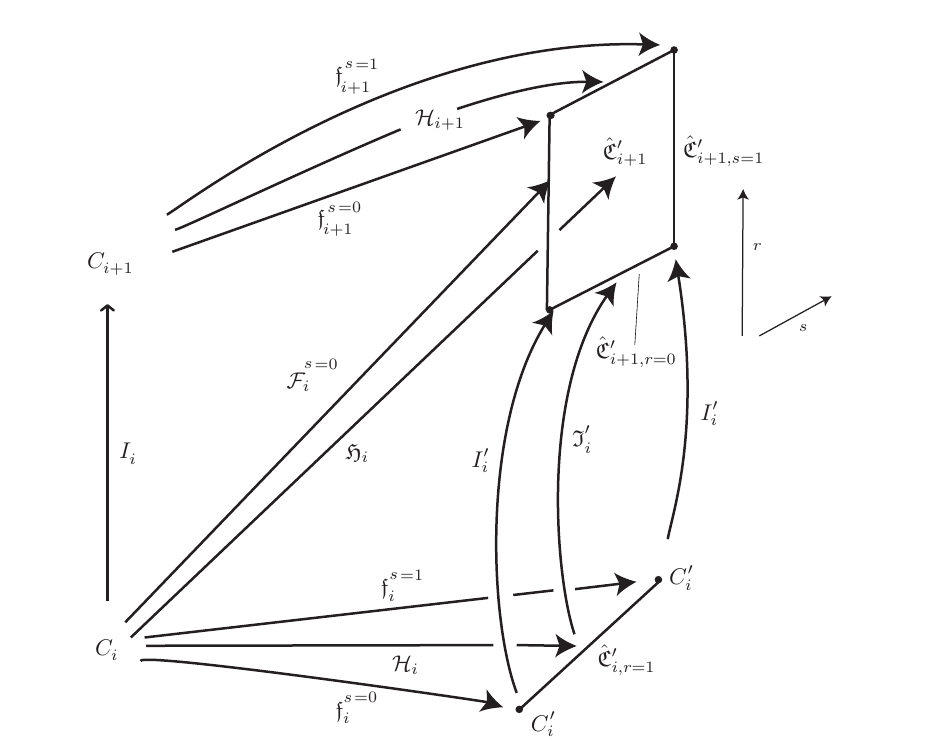
\includegraphics[width=.77\textwidth]{chapters/ch07-transversality/figures/phys-524-figure-7-2-11-math-crop.png}
\par{\renewcommand{\thefigure}{7.2.11}\refstepcounter{figure}
\normalfont\bfseries 图~\thefigure\label{fig:7-2-11}}
\end{minipage}\par\medskip

定义~\ref{def:7-2-204} 的核心是
(7.2.207)：它说明 $\mathfrak H_i$
是同伦的同伦\liftIndex{I275}的一种形式。
以下引理 7.2.208、命题 7.2.211
和定理 7.2.212 表明，
定义~\ref{def:7-2-204} 中的
$A_{(\bar n,\bar k)}$ 代数有向系统
可以提升至 $A_\infty$ 类。

先用引理~\ref{lem:7-2-184} 的
(7.2.185.1)，将
$\{I_i\colon C_i\to C_{i+1}\}$ 与
$\{I'_i\colon C'_i\to C'_{i+1}\}$
提升至 $A_\infty$ 类。
接着提升态射 $\{f_i^{s=s_0}\}$
及其交换误差同伦 $\{\mathcal F_i^{s=s_0}\}$。
为求完整，现重述这一结果，并在下文证明。

\begin{lemma}{7.2.208}\label{lem:7-2-208}
可将 $\{\widehat{\mathfrak C}'_{i,s=s_0}\}$、
$\{f_i^{s=s_0}\}$ 与
$\{\mathcal F_i^{s=s_0}\}$
分别提升为滤过 $A_\infty$ 代数及同态，
使得：

\noindent\textup{(7.2.209)}
$\{\mathcal F_i^{s=s_0}\}$ 提升为
$\{f_i^{s=s_0}\}$ 的提升的
$A_\infty$ 交换误差同伦，
$s_0=0,1$ 分别成立；

\noindent\textup{(7.2.210)}
$\widehat{\mathfrak C}'_{i,s=s_0}$ 的
$\operatorname{Incl}_r$ 提升为滤过
$A_\infty$ 同态，且
$\widehat{\mathfrak C}'_{i,s=s_0}$
提升为 $[0,1]_r\times C'_i$ 的
$A_\infty$ 类模型。
\end{lemma}

这里，模型 $[0,1]\times C$ 的
\emph{提升}，是同时提升其滤过 $A_{n,K}$
代数结构以及 $\operatorname{Eval}$、
$\operatorname{Incl}$，使之成为
$A_\infty$ 类模型。
上述三类提升可能有多种选择；
下文固定其中任意一组。

\begin{proposition}{7.2.211}\label{prop:7-2-211}
可将 $A_{\bar n(\lambda_i),\bar k(\lambda_i)}$
类的 $[0,1]^2\times C'_i$ 模型
$\widehat{\mathfrak C}'_i$
提升为 $A_\infty$ 类模型，
暂不包括关于 $\operatorname{Incl}$ 的断言。
还可将滤过
$A_{\bar n(\lambda_i),\bar k(\lambda_i)}$
同态
$\mathcal I'_i\colon
\widehat{\mathfrak C}'_{i,r=1}
\to\widehat{\mathfrak C}'_{i+1,r=0}$
提升为滤过 $A_\infty$ 同态，
使 (7.2.206) 成为滤过
$A_\infty$ 同态的等式。
\end{proposition}

$\operatorname{Incl}$ 的提升将在
命题 7.2.217 中讨论。
引理~\ref{lem:7-2-208} 和
命题~\ref{prop:7-2-211} 的证明暂缓，
先陈述本小节的主要结果。

\begin{theorem}{7.2.212}\label{thm:7-2-212}
给定 $A_{(\bar n,\bar k)}$ 代数
有向系统的两个态射
$\{f_i^{s=s_0}\}$ 之间的任一同伦
$\{\mathcal H_i\}$，可将它提升为
滤过 $A_\infty$ 同态，
使 (7.2.205) 对 $f_i^{s=s_0}$ 的提升成立。
同样，对依定义~\ref{def:7-2-204}
给定的 $\{\mathcal H_i\}$ 的任一交换误差同伦
$\{\mathfrak H_i\}$，也可作提升，
使 (7.2.207) 成为滤过
$A_\infty$ 同态的等式。
\end{theorem}

\begin{remark}{7.2.213}\label{rem:7-2-213}
定义~\ref{def:7-2-204} 没有假定
$\operatorname{Incl}_s\colon C'_i\to
\widehat{\mathfrak C}'_{i,r=r_0}$
与 $\mathcal I'_i$ 相容。
因此，定理~\ref{thm:7-2-212} 的假设下，
$\operatorname{Incl}_s$ 和
$\operatorname{Incl}\colon C'_i\to
\widehat{\mathfrak C}'_i$
未必能提升为滤过 $A_\infty$ 同态。

事实上，证明定理~\ref{thm:7-2-212} 时
根本不会用到 $\operatorname{Incl}_r$、
$\operatorname{Incl}_s$ 或
$\operatorname{Incl}$。
特别是，即使不假定
$\widehat{\mathfrak C}'_i$ 满足
(7.2.189.6)，定理依然成立。

另一方面，该定理本身并不能推出
$f_i^{s=0}$ 与 $f_i^{s=1}$
滤过 $A_\infty$ 同伦。
原因是 $\widehat{\mathfrak C}'_{i,r=1}$
作为滤过 $A_\infty$ 代数，
未必是 $[0,1]_s\times C'_i$ 的模型；
它按定义~\ref{def:7-2-204}
仅是滤过
$A_{\bar n(\lambda_i),\bar k(\lambda_i)}$
代数层面的模型。
为证明两者滤过 $A_\infty$ 同伦，
还须假定 $\operatorname{Incl}_s$ 与
$\mathcal I'_i$ 之间适当的相容条件，
下述条件 7.2.215 即予以说明。
先看一个说明 $\operatorname{Incl}$
在滤过 $A_\infty$ 同伦理论中作用的例子。
\end{remark}

\begin{example}{7.2.214}\label{ex:7-2-214}
设 $C$ 为滤过 $A_\infty$ 代数，
$\widehat{\mathfrak C}$ 是
$[0,1]_r\times C$ 的模型。
设 $h\colon C\to C$ 是一个
不与恒等映射同伦的同构。
定义新的评价映射
$\operatorname{Eval}'\colon
\widehat{\mathfrak C}\to C$，使
\[
\operatorname{Eval}'_{r=0}
=\operatorname{Eval}_{r=0},
\qquad
\operatorname{Eval}'_{r=1}
=h\circ\operatorname{Eval}_{r=1}.
\]
$\bigl(\widehat{\mathfrak C};
\operatorname{Eval}'_{r=0},
\operatorname{Eval}'_{r=1}\bigr)$
具有 $[0,1]_r\times C$ 模型的各项性质，
唯独没有 $\operatorname{Incl}$。
令 $\mathcal F=\operatorname{Incl}
\colon C\to\widehat{\mathfrak C}$，则
\[
\operatorname{Eval}'_{r=0}\circ\mathcal F
=\mathrm{id},
\qquad
\operatorname{Eval}'_{r=1}\circ\mathcal F=h.
\]
按假设，$h$ 不与恒等映射同伦。
因此，正确界定同伦确实需要
$\operatorname{Incl}$。
\end{example}

为陈述命题 7.2.217，
再定义上述相容条件。
设
\[
\bigl(
\{\mathcal I'_i\colon
\widehat{\mathfrak C}'_{i,r=1}
\to\widehat{\mathfrak C}'_{i+1,r=0}\},
\{\mathfrak H_i\colon C_i\to
\widehat{\mathfrak C}'_{i+1}\}
\bigr)
\]
是两个有向系统态射
$\{f_i^{s=s_0}\}$（$s_0=0,1$）
之间同伦 $\{\mathcal H_i\}$ 的交换误差同伦。
设 $\operatorname{Incl}_s\colon C'_i\to
\widehat{\mathfrak C}'_{i,r=r_0}$
是滤过
$A_{\bar n(\lambda_i),\bar k(\lambda_i)}$
同态，且在同一类同态意义下满足
\[
\operatorname{Eval}_{s=s_0}
\circ\operatorname{Incl}_s=\mathrm{id}.
\]
这样的 $\operatorname{Incl}_s$ 的存在，
是定义~\ref{def:7-2-204} 中
$\widehat{\mathfrak C}'_{i,r=r_0}$
为 $[0,1]_s\times C'_i$ 的
$A_{\bar n(\lambda_i),\bar k(\lambda_i)}$
类模型这一条件的一部分。
\translatornote{原书此处回指“定义 30.204”；
本段所指为定义 7.2.204。}

\begin{statement}{条件}{7.2.215}\label{cond:7-2-215}
对每个 $i$，存在一个滤过
$A_{\bar n(\lambda_{i+1}),\bar k(\lambda_{i+1})}$
代数 $\widetilde{\mathfrak C}'_{i+1}$，
以及滤过
$A_{\bar n(\lambda_i),\bar k(\lambda_i)}$
同态
\[
\widetilde{\mathcal H}_i\colon C'_i
\longrightarrow\widetilde{\mathfrak C}'_{i+1},
\]
满足：

\noindent\textup{(7.2.216.1)}
$\widetilde{\mathfrak C}'_{i+1}$ 是
$[0,1]^2\times C'_{i+1}$ 的滤过
$A_{\bar n(\lambda_{i+1}),\bar k(\lambda_{i+1})}$
代数模型。

\noindent\textup{(7.2.216.2)}
对 $r_0=0,1$，作为
$[0,1]_s\times C'_i$ 的
$A_{\bar n(\lambda_i),\bar k(\lambda_i)}$
类模型，有
$\widetilde{\mathfrak C}'_{i,r=r_0}
=\widehat{\mathfrak C}'_{i,r=r_0}$。
\translatornote{原书右端一律印作
$\widehat{\mathfrak C}'_{i,r=0}$；
这里按 $r_0$ 两端分别相容的要求写出。}

\noindent\textup{(7.2.216.3)}
作为滤过同阶同态，
$\operatorname{Eval}_{r=0}\circ
\widetilde{\mathcal H}_i
=\mathcal I'_i\circ\operatorname{Incl}_s$。

\noindent\textup{(7.2.216.4)}
作为滤过同阶同态，
$\operatorname{Eval}_{r=1}\circ
\widetilde{\mathcal H}_i
=\operatorname{Incl}_s\circ I'_i$。

\noindent\textup{(7.2.216.5)}
作为滤过同阶同态，
$\operatorname{Eval}_{s=s_0}\circ
\widetilde{\mathcal H}_i
=\operatorname{Incl}_r\circ I'_i$。
\end{statement}

粗略地说，条件~\ref{cond:7-2-215}
意指
$\mathcal I'_i\circ\operatorname{Incl}_s
\sim\operatorname{Incl}_s\circ I'_i$，
其中 $\sim$ 是“相对于边界的同伦”。

\begin{proposition}{7.2.217}\label{prop:7-2-217}
考虑两个有向系统态射的同伦
$\{\mathcal H_i\}$ 的交换误差同伦
\[
\bigl(
\{\mathcal I'_i\colon
\widehat{\mathfrak C}'_{i,r=1}
\to\widehat{\mathfrak C}'_{i+1,r=0}\},
\{\mathfrak H_i\colon C_i\to
\widehat{\mathfrak C}'_{i+1}\}
\bigr).
\]
若它满足条件~\ref{cond:7-2-215}，
则 $\operatorname{Incl}_s\liftIndex{I276}\colon C'_i\to
\widehat{\mathfrak C}'_{i,r=r_0}$
与 $\operatorname{Incl}\colon C'_i\to
\widehat{\mathfrak C}'_i$
均可提升为对应提升后滤过
$A_\infty$ 代数之间的同态。
相对于这样得到的
$\operatorname{Incl}_s$ 与
$\operatorname{Incl}$ 的提升，
$\{\widehat{\mathfrak C}'_{i,r=r_0}\}$
及 $\{\widehat{\mathfrak C}'_i\}$
的提升分别成为
$[0,1]_s\times C'_i$ 和
$[0,1]^2\times C'_i$ 的
$A_\infty$ 类模型；这里 $C'_i$
指有向系统 $\{I'_i\colon C'_i\to C'_{i+1}\}$
的滤过 $A_\infty$ 代数提升。
\end{proposition}

命题~\ref{prop:7-2-217} 的证明
留待本小节末尾。

\begin{remark}{7.2.218}\label{rem:7-2-218}
在命题~\ref{prop:7-2-217} 中，
$C'_i$ 与 $\widehat{\mathfrak C}'_i$
的提升上的滤过 $A_\infty$ 结构
已经给定——它们在定理~\ref{thm:7-2-212}
的证明过程中固定，不能再改动。
命题只涉及同态
$\operatorname{Incl}_s$ 与
$\operatorname{Incl}$ 的提升。
\end{remark}

\begin{corollary}{7.2.219}\label{cor:7-2-219}
若定义~\ref{def:7-2-204} 的
交换误差同伦
$\bigl(\{\mathcal I'_i\},\{\mathfrak H_i\}\bigr)$
满足条件~\ref{cond:7-2-215}，
则 $f_i^{s=0}$ 与 $f_i^{s=1}$
滤过 $A_\infty$ 同伦。
\translatornote{原书在此把 $\mathfrak H_i$
的靶写成条件 7.2.215 的辅助模型
$\widetilde{\mathfrak C}'_{i+1}$；
定义 7.2.204 中作为交换误差同伦的
$\mathfrak H_i$ 以
$\widehat{\mathfrak C}'_{i+1}$ 为靶。}
\end{corollary}

推论~\ref{cor:7-2-219} 直接由
定理~\ref{thm:7-2-212} 与
命题~\ref{prop:7-2-217} 得出。
